\chapter{Découvrir les primitives de base}
{ }\hfill\textbf{Niveau:} débutant\\ \\
\noindent
Pour déplacer la tortue sur l'écran, on utilise des commandes prédéfinies appelées \og primitives\fg. Dans ce chapitre, nous allons découvrir certaines primitives de base permettant de piloter la tortue.
\section{Primitives nouvelles utilisées:}
\noindent \begin{enumerate}
\item  \texttt{av nombre}\hspace {4cm } \textcolor{red}{ \texttt{av 50}}\\
Fait avancer la tortue du nombre de pas de tortues indiqué.
\item  \texttt{re nombre}\hspace {4cm } \textcolor{red}{ \texttt{re 100}}\\
Fait reculer la tortue du nombre de pas de tortues indiqué.
\item  \texttt{td nombre}\hspace {4cm } \textcolor{red}{\texttt{td 90}}\\
La tortue tourne vers la droite de l'angle indiqué.
\item  \texttt{tg nombre}\hspace {4cm } \textcolor{red}{ \texttt{tg 45}}\\
La tortue tourne vers la gauche de l'angle indiqué.
\item  \texttt{ve}\hspace {4cm } \textcolor{red}{ \texttt{ve}}\\
Efface l'écran et initialise la tortue au centre de l'écran.
\item  \texttt{mt}\hspace {4cm } \textcolor{red}{ \texttt{mt}}\\
La tortue est visible à l'écran.
\item  \texttt{ct}\hspace {4cm } \textcolor{red}{ \texttt{ct}}\\
Cache la tortue. Peut permettre de rendre l'affichage plus rapide.
\item  \texttt{lc}\hspace {4cm } \textcolor{red}{ \texttt{lc}}\\
Lève le crayon. La tortue ne laisse plus de trait derrière elle lorsqu'elle se déplace.
\item  \texttt{bc}\hspace {4cm } \textcolor{red}{ \texttt{bc}}\\
Baisse le crayon. La tortue écrit lorsqu'elle se déplace.
\item  \texttt{repete nombre liste}\hspace {4cm } \textcolor{red}{ \texttt{repete 5[av 50 td 45]}}\\
Répète les instructions contenues dans la liste le nombre de fois indiqué.
\end{enumerate}
\section{Dessiner un polygone régulier}
\noindent Ici, nous allons apprendre à tracer un carré, un triangle équilatéral, un pentagone régulier etc
\subsection{Le carré}
\begin{center}
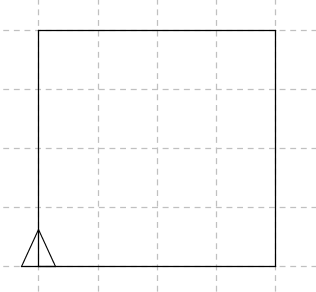
\includegraphics{images/bases-carre.png}
\end{center}
\noindent Un carreau représente 50 pas de tortue. Pour dessiner le carré ci-contre, on va donc taper:
\begin{verbatim}
av 200 td 90 av 200 td 90 av 200 td 90 av 200 td 90
\end{verbatim}
On s'aperçoit ainsi que l'on répète $4$ fois la même instruction d'où une syntaxe plus rapide:
\begin{verbatim}
repete 4[av 200 td 90]
\end{verbatim}
\subsection{Le triangle équilatéral}
\begin{center}
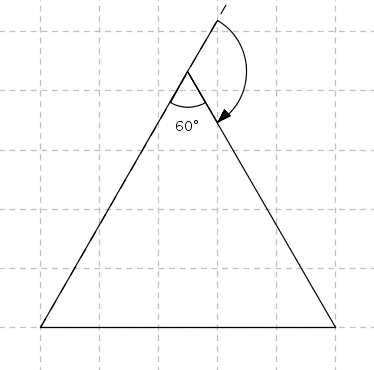
\includegraphics{images/bases-triangle.png}
\end{center}
\noindent Ici, un carreau représente 30 pas de tortues. Nous allons voir ici comment tracer ce triangle équilatéral de 150 pas de tortue de côté.\\ \\
La commande ressemblera à quelque chose du style: 
\begin{verbatim}
repete 3[av 150 td ....]
\end{verbatim}
Reste à déterminer le bon angle. Dans un triangle équilatéral, les angles valent tous 60 degrés. Comme la tortue doit tourner à l'extérieur du triangle. L'angle vaudra 180-60=120 degrés. La commande est donc:
\begin{verbatim}
repete 3[av 150 td 120]
\end{verbatim}
\subsection{L'hexagone}
\begin{center}
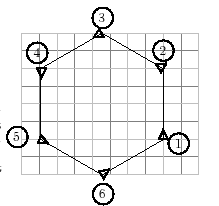
\includegraphics{images/bases-hexagone.png}
\end{center}
\noindent Ici, un carreau représente 20 pas de tortues.\\
\begin{verbatim}
repete 6[av 80 td ....]
\end{verbatim}
On s'aperçoit que lors de son déplacement, la tortue effectue en fait un tour complet sur elle même. (Elle part orientée vers le haut puis revient dans cette position). Cette rotation de 360 degrés s'effectue en 6 étapes.\\
 Par conséquent, à chaque fois, elle tourne de $\dfrac{360}{6}=60$\degre. \\ \\
La commande est donc: \texttt{repete 6[av 80 td 60]}

\subsection{Tracer un polygone régulier en général}
\noindent En fait, en réitérant le petit raisonnement précédent, on s'aperçoit que pour tracer un polygone à $n$ côtés, l'angle s'obtiendra en divisant 360 par $n$. Par exemple:\begin{itemize}
\item Pour tracer un pentagone régulier de côté 100:
\begin{verbatim}
repete 5[av 100 td 72]    (360:5=72)
\end{verbatim}
\item Pour tracer un ennagone régulier (9 côtés) de côté 20:
\begin{verbatim}
repete 9[av 20 td 40]    (360:9=40)
\end{verbatim}
\item Pour tracer un euh... 360-gone régulier de côté 2: (ça ressemble fortement à un cercle, ça!)
\begin{verbatim}
repete 360[av 2 td 1]  
\end{verbatim}
\item Pour tracer un heptagone de côté 120:
\begin{verbatim}
repete 7[av 120 td 360/7]
\end{verbatim}
\end{itemize}

\section{Enregistrer une procédure}
\noindent Pour éviter d'avoir à retaper à chaque fois les instructions pour
dessiner un carré, un triangle ... on peut définir des instructions personnelles appelées \og procédures \fg. Une procédure commence par le mot-clé \texttt{pour} et se termine par le mot-clé \texttt{fin}. On ouvre l'éditeur, on tape par exemple

\begin{verbatim}
pour carre
repete 4[av 100 td 90]
fin
\end{verbatim}
puis on ferme l'éditeur en enregistrant les modifications en cliquant sur le bouton tortue.  Maintenant à chaque fois que l'on tape \texttt{carre}, un carré apparaît à l'écran!

\section{Exercice ...}
\noindent
Un petit carreau représente 10 pas de tortue.\\
Essayer de réaliser le dessin ci-dessous en définissant huit procédures:
\begin{itemize}
\item Une procédure \og \texttt{carre} \fg{} qui tracera le carre de base
de la maison.
\item Une procédure \og \texttt{tri} \fg{} qui tracera le triangle équilatéral
représentant le toit de la maison.
\item Une procédure \og \texttt{porte} \fg{} qui tracera le rectangle
représentant la porte.
\item Une procédure \og \texttt{che} \fg{} qui tracera la cheminée
\item Une procédure \og \texttt{dep1} \fg{} qui permettra à la tortue
de se déplacer de la position A à la position B.
\item Une procédure \og \texttt{dep2} \fg{} qui permettra à la tortue
de se déplacer de la position B à la position C.
\item Une procédure \og \texttt{dep3} \fg{} qui permettra à la tortue
de se déplacer de la position C à la position D. (Attention, il faudra
peut-être lever le crayon de la tortue...)
\item Une procédure \og \texttt{ma} \fg{} qui permettra de tracer la maison
en entier en s'aidant de toutes les autres procédures.
\end{itemize}
\label{maison}
\begin{center}
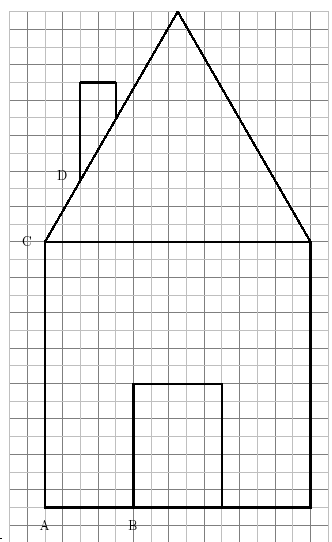
\includegraphics[scale=0.6]{images/bases-maison.png}
\end{center}